\subsection{Threat Model}

\begin{figure}
    \centering
        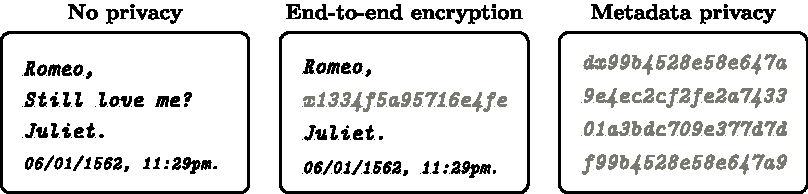
\includegraphics[width=\textwidth]{metadata-privacy.pdf}
\caption{Differences between non-E2E, E2E, and Metadata-Hiding protocols for a message from Romeo to Juliet.}
\label{fig:metadataprivacy}
\end{figure}

%\begin{table*}[t]
%\centering
%another version below
%\begin{tabular}{||c c c c c c||} 
% \hline
%  Attacker compromises $\cdots$ & Anysphere & Signal & Skiff & Wickr & Onion  \\
% \hline
% Attacker listens on the internet & \checkmark & \checkmark & \checkmark & \checkmark \\ 
% \hline
% Attacker compromises & \checkmark & & & \checkmark & \checkmark \\
% \hline
% Skiff & \checkmark &  &  & & \checkmark\\
% \hline
% Wickr & \checkmark & & & \checkmark & \checkmark\\
% \hline
% Onion & \checkmark & *\footnote{\label{onion}Only guaranteed for non-global adversary} & &\checkmark&\checkmark\\
% \hline
%\end{tabular}
%\caption{Comparing when}
%\end{table*}


\xxx{add an illustration of a walled garden, with the walls containing only your computer and your friends' computers}

%Touch on: server, friends, client-side computer, etc.

\xxx{Figure out a better format here. See e.g. Skiff's whitepaper.}

1. \textbf{Compromised Server}: We do not have any trust in the server. Similar to most PIR schemes(for example \cite{ahmad2021addra}, \textsection 2.2), our threat model assumes a global adversary who has control over all the servers, and can observe and manipulate all network traffic.

2. \textbf{Compromised Strangers}: Similarly, we assume that the adversary has control over all non-friend clients, and can observe and manipulate all network traffic from and to these clients.

3. \textbf{Trusted Friends}: In \cite{angel2018s}, Angle, Lazar and Tzialla describes the compromised friend(CF) attack on a general meta-data private messaging system, which shows that perfectly hiding metadata while not trusting the user's friends is computationally prohibitive. In our threat model, a user trusts that their devices, as well as the devices of all their friends, are uncompromised and running our client code. \xxx[stzh]{In the future, we would look into measures for handling friend compromises?} 

4. \textbf{Secure Cryptographical Primitives}: Our threat model assumes the security of the standard cryptography primitives we use, including Microsoft SEAL's BFV cryptosystem and libsodium's AEAD cryptosystem. 



\subsection{Non-goals}
1. \textbf{Not a cryptocurrency}: Anysphere's underlying PIR algorithm is unrelated to blockchains and cryptocurrencies.

2. \textbf{Not a plugin}: Anysphere relies on a dedicated PIR server to work. Therefore, Anysphere is not compatible with existing messaging systems like Messenger or Signal, and does not work like a google chrome extension to these apps.

3. \textbf{Not steganographic}: Anysphere does not make an attempt to hide who's using our service. \xxx[sualeh]{This might change in the future?}

